\documentclass{beamer}

\usetheme{boxes}


\usecolortheme[RGB={34,170,34}]{structure}
\usepackage{amsmath}
\usepackage{amssymb}
\usepackage{graphics}
\usepackage{multicol}
\usepackage{color}
\usepackage[absolute,overlay]{textpos}

\usepackage{framed,color}
\definecolor{shadecolor}{rgb}{255,127,0}
\setbeamertemplate{itemize item}[circle]

\definecolor{verde}{RGB}{34,170,34}


\setbeamercolor{uppercolgreen}{fg=white,bg=verde!90}
\setbeamercolor{lowercolgreen}{fg=black,bg=verde!20}



%%%%%%%%%%%%%%%%%%%%%%%%%%%%%%%%%%%


\title[Mercurial]{Version Control}

\subtitle[]{EOAS Software Carpentry Workshop }
\date[Sep 2015]{September 23rd, 2015}
% double-hyphen command to make -- render as separate dashes instead
% of as an m-dash
\renewcommand{\dh}{{-}{-}}



\begin{document}

\section*{Mercurial (hg)}

\begin{frame}[plain]
\titlepage
\end{frame}

\subsection*{Automated Version Control}
\begin{frame}
\frametitle{Automated Version Control}
\begin{block}{Learning Goals}
\begin{enumerate}
\item Understand the benefits of an automated version control system.
\item Understand the basics of how Mercurial works
\end{enumerate}
\end{block}
\end{frame}

\begin{frame}
\begin{columns}
\column{0.6\textwidth}
\resizebox{!}{\textheight}{
\includegraphics{fig/phd101212s.png}}
\column{0.4\textwidth}
"Piled Higher and Deeper" by Jorge Cham, http://www.phdcomics.com
\end{columns}
\end{frame}

\begin{frame}
\frametitle{Automated Version Control}
\begin{block}{Changes are saved sequentially}
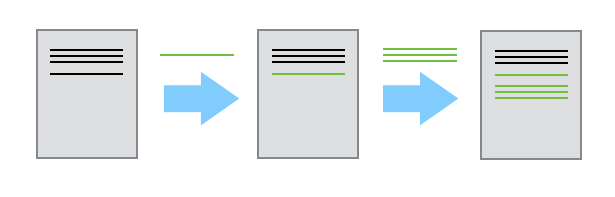
\includegraphics[scale=0.65]{fig/play-changes.png}
\end{block}
\end{frame}

\begin{frame}
\frametitle{Automated Version Control}
\begin{block}{Different versions can be saved}
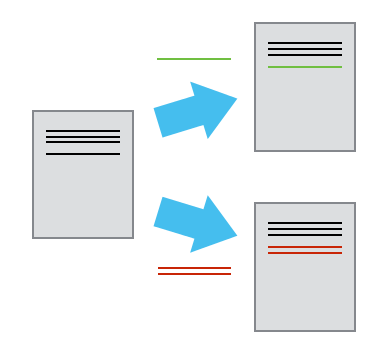
\includegraphics[scale=0.8]{fig/versions.png}
\end{block}
\end{frame}

\begin{frame}
\frametitle{Automated Version Control}
\begin{block}{Multiple versions can be merged}
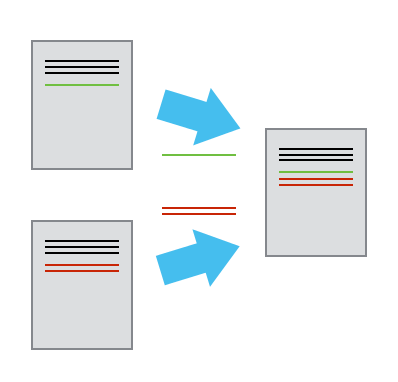
\includegraphics[scale=0.8]{fig/merge.png}
\end{block}
\end{frame}

\subsection*{Configuring Mercurial}
\begin{frame}[fragile]
\frametitle{Configuring Mercurial}
%\begin{block}{Learning Goal}
%\begin{enumerate}
%\item Explain what configuration steps are required the first time Mercurial is used on a computer.
%\end{enumerate}
%\end{block}

\texttt{\$ EDITOR=nano hg config --edit}

\begin{verbatim}
[ui]
username = Vlad Dracula <vlad@tran.sylvan.ia>
editor = nano

[extensions]
color =

[color]
mode = win32
\end{verbatim}

\end{frame}


\subsection*{Creating a Repository}
\begin{frame}
\frametitle{Creating a Repository}
\begin{block}{Learning Goal}
\begin{enumerate}
\item Explain how to initialize a new Mercurial repository.
\end{enumerate}
\end{block}

\begin{block}{Lesson Commands}
\begin{multicols}{2}
\begin{itemize}
\item mkdir forecast
\item cd forecast
\item hg init
\item ls -a
\item hg verify
\end{itemize}
\end{multicols}
\end{block}
\end{frame}

\subsection*{Tracking Files}
\begin{frame}
\frametitle{Tracking Files}
\begin{block}{Learning Goals}
\begin{enumerate}
\item Display the version control status of files in a repository and explain what those statuses mean.
\item Add files to Mercurial's collection of tracked files.
\item Record metadata about changes to a file.
\item Display the history of changes to files in a repository and explain the metadata that is recorded with each changeset.
\end{enumerate}
\end{block}
\begin{block}{Lesson Commands}
\begin{multicols}{2}
\begin{itemize}
\item nano plan.txt
\item hg status
\item hg add plan.txt
\item hg commit -m "Starting to plan the daily NEMO forecast system."
\item hg log
\end{itemize}
\end{multicols}
\end{block}
\end{frame}

\subsection*{Making Changes}
\begin{frame}
\frametitle{Making Changes}
\begin{block}{Learning Goals}
\begin{enumerate}
\item Display the uncommitted changes that have been made to tracked files.
\item Go through the modify-commit cycle for single and multiple files.
\end{enumerate}
\end{block}
\begin{block}{Lesson Commands}
\begin{multicols}{2}
\begin{itemize}
\item nano plan.txt
\item hg status
\item hg diff
\item hg commit -m "Note about atmospheric forcing."
\item nano biblio.txt
\item hg add biblio.txt
\item hg commit -m "Added citation" biblio.txt
\end{itemize}
\end{multicols}
\end{block}
\end{frame}

\begin{frame}
\frametitle{Exercise}
Create a new Mercurial repository on your computer called bio. Write a three-line biography for yourself in a file called me.txt, commit your changes, then modify one line and add a fourth and display the differences between its updated state and its original state.
\end{frame}



\subsection*{Exploring History}
\begin{frame}
\frametitle{Exploring History}
\begin{block}{Learning Goals}
\begin{enumerate}
\item Compare files with older versions of themselves.
\item Display the changes that were made to files in a previous changeset.
\end{enumerate}
\end{block}
\begin{block}{Lesson Commands}
\begin{multicols}{2}
\begin{itemize}
\item hg diff \dh rev 1:2 plan.txt
\item hg diff -r 0:2 plan.txt
\item hg diff \dh change 1
\end{itemize}
\end{multicols}
\end{block}
\end{frame}


\subsection*{Recovering Old Versions}
\begin{frame}
\frametitle{Recovering Old Versions}
\begin{block}{Learning Goals}
\begin{enumerate}
\item Restore older versions of files.
\item Use configuration aliases to create custom Mercurial commands.
\end{enumerate}
\end{block}
\begin{block}{Lesson Commands}
\begin{multicols}{2}
\begin{itemize}
\item nano plan.txt
\item hg revert plan.txt
\item hg revert \dh rev 0 plan.txt
\item hg status
\end{itemize}
\end{multicols}
\end{block}
\end{frame}

\subsection*{Ignoring Things}
\begin{frame}[label=ignore]
\frametitle{Ignoring Things}
\begin{block}{Learning Goal}
\begin{enumerate}
\item Configure Mercurial to ignore specific files and explain why it is sometimes useful to do so.
\end{enumerate}
\end{block}
\begin{block}{Lesson Commands}
\begin{itemize}
\item mkdir inprogress
\item touch plan.txt$~$ inprogress/a.out inprogress/b.out
\item hg status
\item nano .hgignore
\item hg status \dh ignored
\end{itemize}
\end{block}
\end{frame}

\begin{frame}[fragile]
\frametitle{.hgignore}
\begin{verbatim}
syntax: glob
*~
inprogress/
\end{verbatim}
\end{frame}

\againframe{ignore}


\begin{frame}[label=remote-repos]
  \frametitle{Remote Repositories}
  \begin{block}{Learning Goals}
    \begin{enumerate}
      \item Explain what remote repositories are and why they are useful.
      \item Explain what happens when a remote repository is cloned.
      \item Explain what happens when changes are pushed to or pulled from a remote repository.
    \end{enumerate}
  \end{block}
  \begin{block}{Lesson Commands}
    \begin{itemize}
      \item hg push
      \item hg config \dh local
      \item hg paths
      \item hg pull
    \end{itemize}
  \end{block}
\end{frame}


\begin{frame}
  \frametitle{Remote Repositories}
  \begin{block}{Local and Bitbucket Repos After 1st Push}
    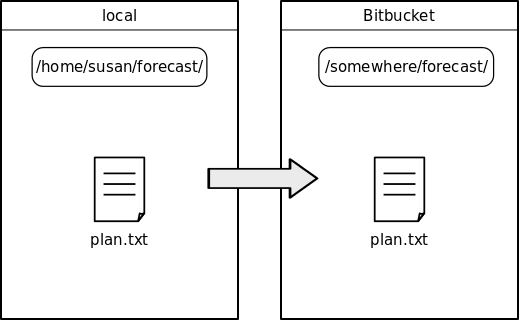
\includegraphics[scale=0.55]{fig/bitbucket-repo-after-first-push.png}
  \end{block}
\end{frame}


\againframe{remote-repos}


\begin{frame}[label=clones]
  \frametitle{Working with Clone Repositories}
  \begin{block}{Learning Goals}
    \begin{enumerate}
      \item Explain how to push, pull, update files, and update metadata among clones of a repository.
      \item Display a simple visualization of the state of a repository and explain how updating the repository affects its state.
    \end{enumerate}
  \end{block}
  \begin{block}{Lesson Commands}
    \begin{itemize}
      \item hg clone
      \item hg add
      \item hg commit
      \item hg push
      \item hg pull
      \item hg log \dh graph
      \item hg update
    \end{itemize}
  \end{block}
\end{frame}


\begin{frame}
  \frametitle{Working with Clone Repositories}
  \begin{block}{After Creating work and home Clones}
    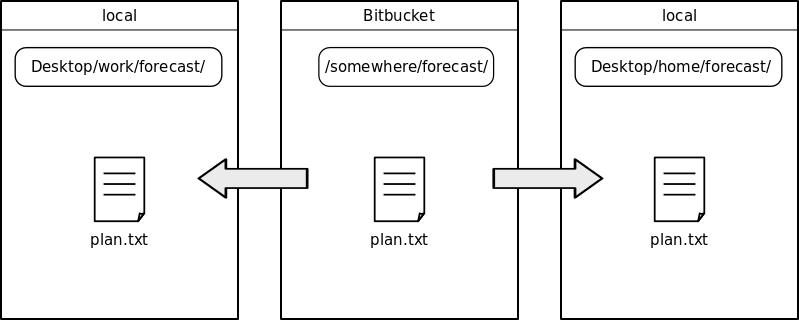
\includegraphics[scale=0.40]{fig/hg-after-home-work-clones.png}
  \end{block}
\end{frame}


\begin{frame}
  \frametitle{Working with Clone Repositories}
  \begin{block}{After Pushing Change from work Clone}
    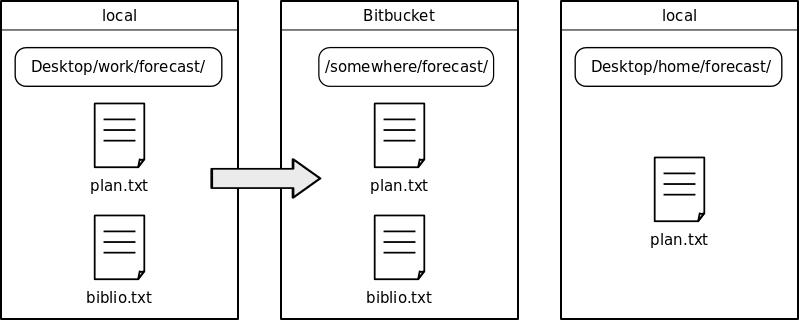
\includegraphics[scale=0.40]{fig/hg-after-change-to-work-clone.png}
  \end{block}
\end{frame}


\begin{frame}
  \frametitle{Working with Clone Repositories}
  \begin{block}{After Pulling Change into home Clone}
    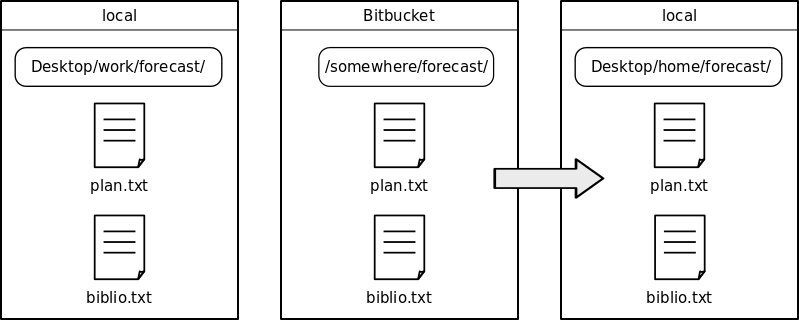
\includegraphics[scale=0.40]{fig/hg-after-pulling-to-home-clone.png}
  \end{block}
\end{frame}


\againframe{clones}


\begin{frame}
  \frametitle{Collaboration}
  \begin{block}{Learning Goals}
    \begin{enumerate}
    \item Explain the differences between public and private repositories on Bitbucket.
    \item Configure user and group access settings for Bitbucket repositories.
    \end{enumerate}
  \end{block}
\end{frame}


\begin{frame}[label=merging]
  \frametitle{Merging Changes from Different Clones}
  \begin{block}{Learning Goals}
    \begin{enumerate}
    \item Explain how Mercurial handles changes that make a repository's history diverge.
    \item Explain what merges are.
    \end{enumerate}
  \end{block}
  \begin{block}{Lesson Commands}
    \begin{multicols}{2}
      \begin{itemize}
        \item hg commit
        \item hg push
        \item hg pull
        \item hg heads
        \item hg log -G
        \item hg merge
        \item hg status
        \item hg diff
        \item hg summary
      \end{itemize}
    \end{multicols}
  \end{block}
\end{frame}


\begin{frame}[label=merge-conflicts]
  \frametitle{Merge Conflicts}
  \begin{block}{Learning Goals}
    \begin{enumerate}
    \item Explain what merge conflicts are and when they can occur.
    \item Resolve conflicts resulting from a merge using the KDiff3 tool.
    \end{enumerate}
  \end{block}
  \begin{block}{Lesson Commands}
    \begin{itemize}
      \item hg incoming
      \item hg pull
      \item hg update
      \item hg log \dh graph
      \item hg merge \dh tool=kdiff3
    \end{itemize}
  \end{block}
\end{frame}

\end{document}

